\documentclass[a4paper,12pt,twoside]{report}

\usepackage[french]{babel}  % Pour le français
\usepackage[utf8]{inputenc} % Pour taper les caractères accentués
\usepackage{amssymb}
\usepackage{amsmath}  % Ces trois paquets donnent accès à 
\usepackage{amsfonts} % des symboles et formulations
\usepackage{amstext}  % mathématiques
\usepackage{hyperref} % Permet de faire automatiquement des liens dans les
                      % documents
                      
\usepackage{mathrsfs}
\usepackage{float}
\usepackage{graphicx} % Permet d'insérer des images
\DeclareGraphicsExtensions{.png} % Mettre ici la liste des extensions des
                                 % fichiers images

% On peut choisir la police en utilisant un paquet 
%\usepackage{newcent}
\usepackage{lmodern}
%\usepackage{cmbright} % Computer Modern Bright

% Une des nombreuses manière de modifier les marges par défaut
\usepackage{geometry}
\geometry{vmargin=2cm,hmargin=2.5cm,nohead}
\newcommand{\oa}[2][]{#1|_{#2}}
% On peut redéfinir certaines longueurs, par exemple l'espacement entre les
% paragraphes:
\setlength{\parskip}{0.25cm}
\usepackage{geometry}
\geometry{vmargin=2cm,hmargin=2.5cm,nohead}
% Quelques définitions 
\def \kk {{\mathbb K}}
\def \rr {{\mathbb R}} % L'ensemble R
\def \cc {{\mathbb C}} % L'ensemble C
\def \nn {{\mathbb N}} % L'ensemble N
\def \zz {{\mathbb Z}} % L'ensemble Z
\def \H {{\mathscr{H}}} % Espace d'hilbert
%\newcommand{\at}[2][]{#1|_{#2}}
\usepackage[overload]{empheq}
\usepackage{graphicx, wrapfig, lipsum}
% Les informations de la page de titre (page de titre séparée pour un 'report').
% \thanks: permet de mettre une note de bas de page pour l'auteur
% \href: insère un lien, ici vers l'application 'mailto'
% \tt: police monospace
%\date{\today} % \today pour la date courante 




\usepackage{pstricks-add}

\begin{document}

%\maketitle % Page de titre automatique à partir des infos ci-dessus


\begin{titlepage}
	
	\newcommand{\HRule}{\rule{\linewidth}{0.5mm}} 
	\center
	
	
	\textsc{\LARGE Université de Bordeaux }\\[1.5cm] % Name of your university/college
	\textsc{\Large Deep Learning}\\[0.5cm] % Major heading such as course name
	%\textsc{\large et Ouverture au Monde Professionnel }\\[0.5cm] % Minor heading such as course title
	
	\HRule \\[0.4cm]
	{ \huge \bfseries Deep Neural Networks ( lab2 )
}\\[0.4cm] % Title of your document
	\HRule \\[1.5cm]
	
	\hfill
	
	\begin{figure}[H]
	\centering
	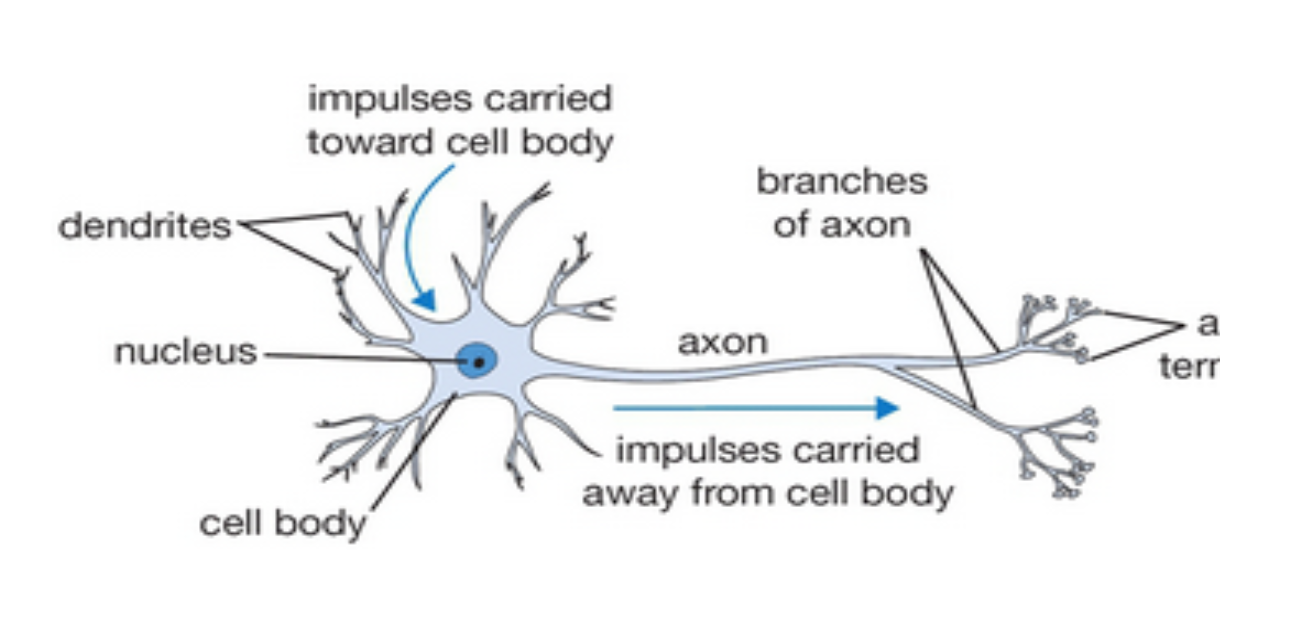
\includegraphics[scale=0.6]{Bio_Neuron.png} 
	\end{figure}

	
	\begin{minipage}{0.4\textwidth}
		\begin{flushleft} \large
			Abderrahim \textsc{Serghini}\\
		\end{flushleft}
	\end{minipage}
	~
	
	
	{\large \today}\\[2cm]
	
\end{titlepage}

\newpage

\paragraph{One Neuron : }

Following the course, we first used the architecture of one neuron : 

\begin{figure}[H]
\centering
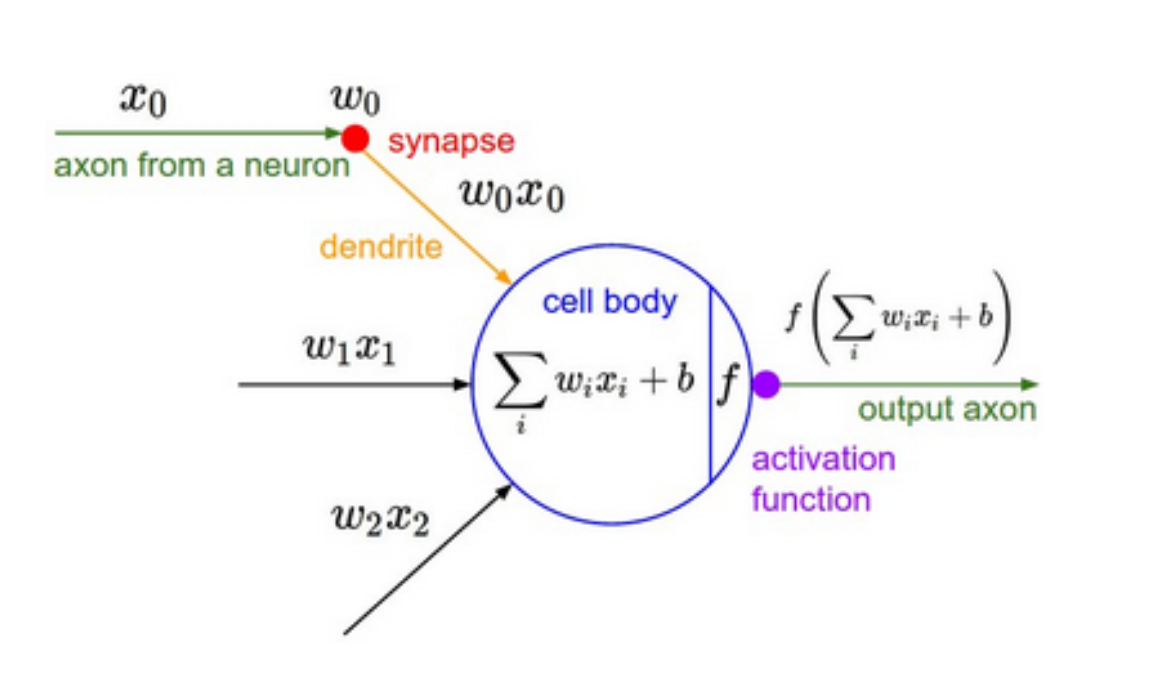
\includegraphics[scale = 0.6]{One_neuron_arch.png}
\caption{A simple architecture of a neural network}
\end{figure}

Where we take the pixels of the image as the input, the weights are taken as a random vector while we f is the sigmoid functions :
$$ f(x)= \sigma(x) = \frac{1}{1 + e^{-x}} $$
And Y as the output as $\sigma(w^Tx + b)$
 
\subparagraph{Forward Propagation : }

The mathematical expression for the loss function using the cross entropy is :
$$ L(x) = - \sum Y log(\hat{Y}) + \sum (1 - Y)log(1-\hat{Y})$$

\subparagraph{Backward Propagation :}

The derivative of L in accordance to its component W ( using the chain rule, and m being the number of examples )
$$\frac{dL}{dW} = \frac{1}{m} (\hat{Y} - Y).X^T $$
We also need the derivative of b in which we get using the same rule :
$$ db = \frac{1}{m} \sum (\hat{Y} - Y)  $$

\subparagraph{Results :}
Testing the model for 500 epochs we get the following result :
\begin{figure}[H]
\centering
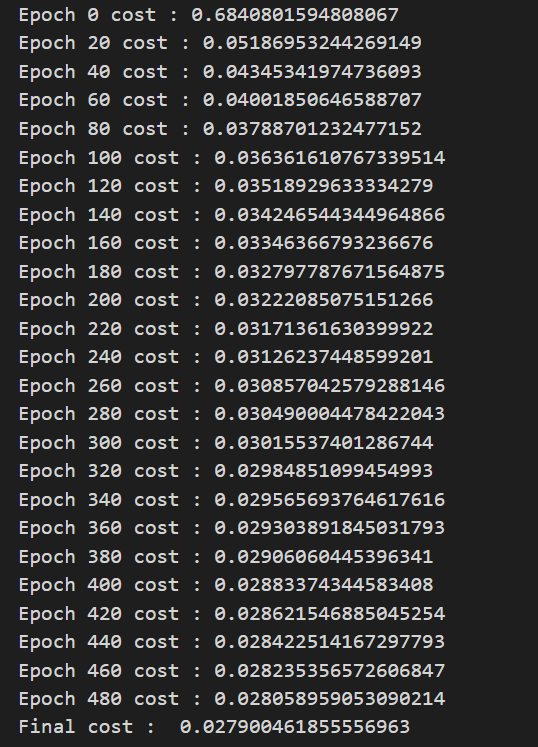
\includegraphics[scale = 0.6]{lab2_1_cost.png}
\caption{Test using the one Neuron model, the cost being calculated each 20th iteration}
\end{figure}

\paragraph{A Hidden layer :}

With the same activation function and the loss function, we can add another layer and calculate the derivative once again with the same method.
We get then the following results :

\begin{figure}[H]
\centering
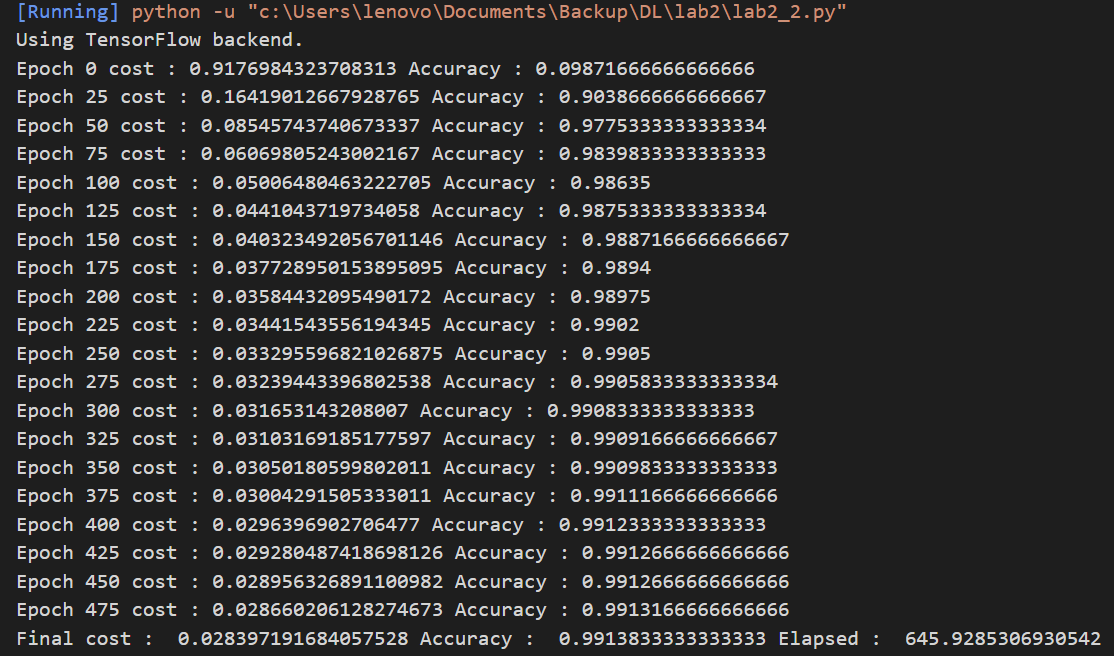
\includegraphics[scale = 0.6]{lab2_2_cost_acc_64.png}
\caption{Test adding a Hidden layer of 64 elements achieving a 99,13 \% accuracy}
\end{figure}

The results do not change drastically when adding more elements to the hidden layer : 

\begin{figure}[H]
\centering
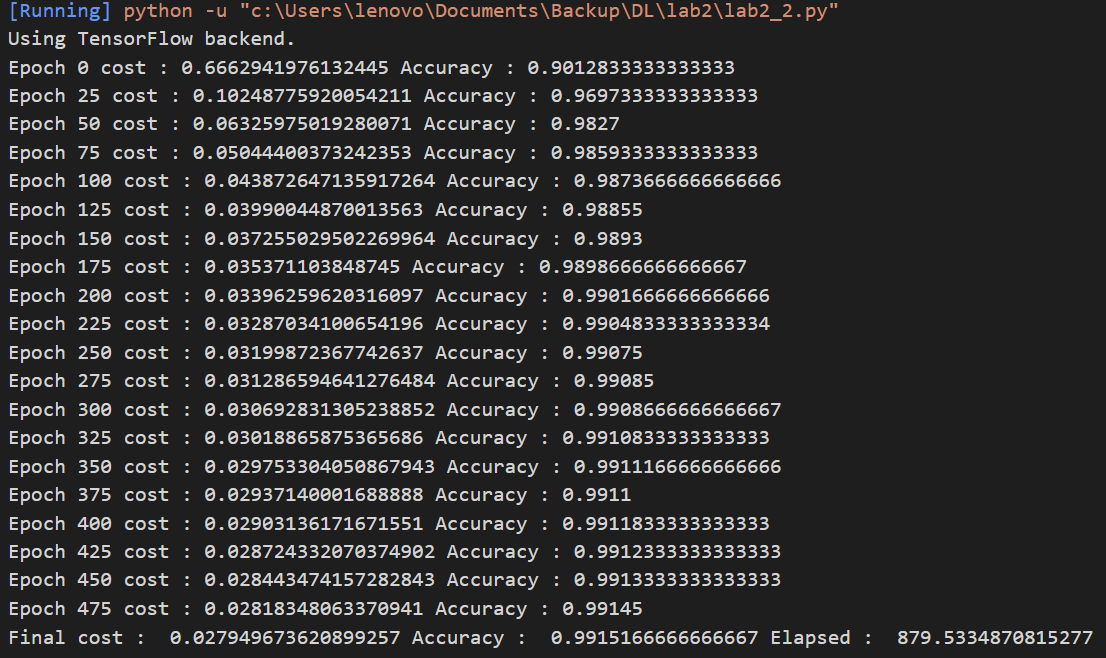
\includegraphics[scale = 0.6]{lab2_2_cost_acc.png}
\caption{Test adding a Hidden layer of 128 elements achieving a 99,15 \% accuracy}
\end{figure}

\paragraph{Multi neural network}

\begin{figure}[H]
\centering
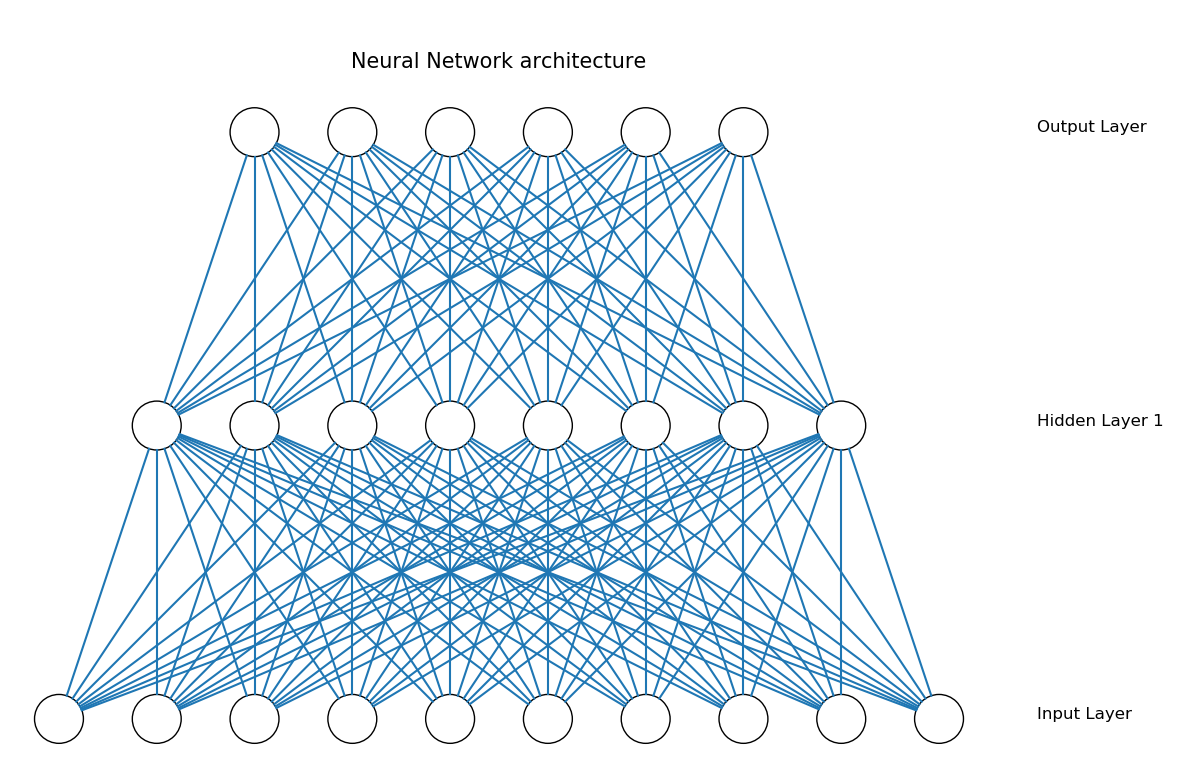
\includegraphics[scale = 0.6]{Figure_1.png}
\caption{Architecture of the neural network}
\end{figure}

Above is the architecture of our neural network, composing of an input of 728 elements, A hidden layer of 64 elements and an output of 10 elements ( representing the hot encoding of the numbers ranging from 0 to 9 )

After running the test we get the following result :

\begin{figure}[H]
\centering
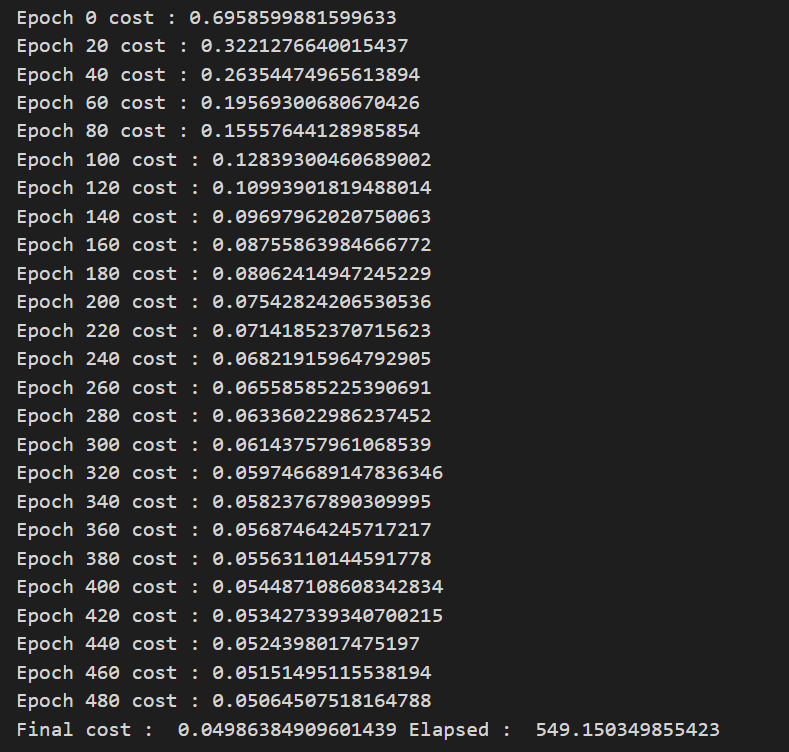
\includegraphics[scale = 0.6]{lab2_3_cost_64.png}
\caption{test of multi neural network }
\end{figure}


\end{document}